\documentclass[a4paper]{article}
\usepackage[letterpaper, margin=1in]{geometry} % page format
\usepackage{listings} % this package is for including code
\usepackage{graphicx} % this package is for including figures
\usepackage{amsmath}  % this package is for math and matrices
\usepackage{amsfonts} % this package is for math fonts
\usepackage{tikz} % for drawings
\usepackage{hyperref} % for urls
\graphicspath{ {./images/} }

\title{CSI 4352 Project Writeup: Trump Speech 2024}
\author{Par Wilkinson}
\date{12/4/2020}

\begin{document}
\lstset{language=Python}

\maketitle

\section{Resources}
Colab Link: $https://colab.research.google.com/drive/16p6TKbSyJ0_0XBTGIFQe5Gb7tQ3cHMSQ?usp=sharing$ \\
Dataset Required:  $https://www.kaggle.com/christianlillelund/donald-trumps-rallies$ \\
LaTeX Source Files: $https://github.com/ParWilkinson/ProjectWriteupLatex$ 

\section{Abstract}

This paper summarizes the results of my research on using deep learning for text generation, and my attempts to implement a model that generates text in the form of a Donald Trump campaign speech. I ran into a few difficulties dealing with limited resources on Google colabs, but I managed to get some interesting results from some of the models I trained. 

\section{Introduction}

In order to generate a transcription in the flavor of a Donald Trump speech, I've gathered a few research papers on text generation. This paper describes some of the methods used by other researchers to generate stories, context-based text, and text in general. In my project, I combine these findings to train as realistic and as Trump-esque a model as I can while remaining conscious of overfitting and other issues.

\section{Background}

A key point in one of the papers I read is that the best models for text generation are the ones suited for modeling sequence data \cite{Z}. Considering that the desired output of text generation is something meaningful and that a model learning to produce random gibberish isn't interesting, it's clear that the task of text generation is sequential in nature. When forming sentences randomly, the previous chosen words are highly important in producing the next word. It's for this reason that plain feed-forward fully-connected encoder-decoder models are not recommended, but instead RNN or CNN-based models perform well. \\

\noindent 
A few of the other papers I read deal specifically with using LSTM-RNN models for text generation. Long short term memory (LSTM) networks work to remedy the vanishing gradient problem due to back propagation \cite{C}. LSTM networks are useful especially for text generation due to their ability to "remember" values for long and short durations of time \cite{SS}. The "Story Scrambler" paper written by various authors explains the step by step process its Story Scrambler System uses to process input, create and train the neural network, and then produce the story \cite{SS}.  This approach operates at the word level, meaning that the model predicts the next expected word given a sequence of words. \\

\noindent
An alternative text generation method is generating text at the character level. While generally not as used as word-level text generation, it's possible to generate relevant text at the character-level with a well constructed and well trained model \cite{CL}. This gives the model a lot more freedom to create gibberish due to not being restricted to a limited vocabulary, but the approach is also a bit more interesting as the model is trained with no prior understanding of words or limitations. \\

\noindent
Another interesting text generation approach I read about used a Variational Autoencoder model where the encoder and decoder are each LSTM networks \cite{VAE}. I found that to be an intuitive way to go about text generation, because Variational Autoencoders are really useful for learning a latent representation of data and then using the decoder portion to generate new data. I didn't implement this model in my experiments with Trump text generation, as the method for generating a new text sequence in a way that combines next-word-prediction and a VAE would be difficult. \\

\noindent
It's also possible to improve upon text generator performance through utilizing Generative Adversarial Networks, by training a generator that produces high quality samples for text generation training \cite{GAN}. One of the main issues with getting higher quality text generation is that the training data might not cover many of the valid sequences of words possible, so it's unlikely the model will ever generate those subsequences. This isn't especially useful for this project, since the goal was to mimic a specific person's mannerisms, but in other types of text generation applications it might be really valuable to utilize GANs for data augmentation purposes. \\

\section{Methodology}

The most popular dataset on Kaggle pertaining to what Trump has said is of course an archive of his tweets, but that was not used for this project as tweets don't necessarily flow the same way speeches do. Because this model seeks to generate text emulating Trump's campaign speeches, the most useful dataset I could find is an archive of speeches given by Trump at 35 of his rallies. This data is simply in the form of text documents containing a full length transcription of the speech for that particular rally. The dataset used can be found at: https://www.kaggle.com/christianlillelund/donald-trumps-rallies \\

\noindent
In the creation of this project, I trained and evaluated a few different LSTM networks built for text generation at the word-level. In order to train the models, I first had to prepare the input data which consisted of 35 text files containing text transcriptions of Donald Trump speeches. The first thing I did was concatenate the text files into a single string, before trimming all the quotation marks to avoid confusing the model. Quotation marks are either attached to the front or back of words and weren't used much in all of the text files, so to avoid confusing the model I cut them out of the input text. The next thing I did was insert a space before all types of punctuation, to ensure the model would treat punctuation as separate words to be chosen in sequences. This should allow the model to freely form sentences. \\

\noindent
After manipulating the data, the complete text length came out to be $2083799$ characters. Next, I obtained from the text the set of unique words, which came out to be $10899$ in length. This was used to create two maps, one mapping each word to a unique id and another table mapping the id back to the word. Next, I split the data into sequences of length 80. Unfortunately due to the RAM limitations of Google colabs, the more sequences I split the text into, the more likely the session was to break the RAM limit and crash. For most models, I ended up training with a sequence length of 80 which gave only 8000 sequences for training. \\

\noindent
Next, to prepare for model training I created a callback to generate a story every X amount of epochs, set by $benchmark\_epoch$. Randomly seeded text generation is performed by picking a random sequence of words from the text and having the trained model predict the next word in the sequence over and over until a fully new sequence has been generated.  \\

\noindent
Multiple different model approaches were tested in this project, all of them sharing in common the same Input layer which takes the sequence of words, at least one LSTM layer, and a Dense layer outputting the predicted next word from the word-set.

\section{Experiments}
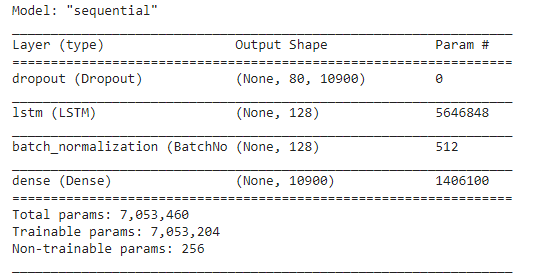
\includegraphics{model1}
The first model I tried to use consisted of only one LSTM layer with Dropout and Batch Normalization. The text generation results for this model were really poor, and the loss wouldn't go low enough to form very coherent sentences in the stories generated. This is a text sample from that model: \\ \\
?? because that last people that because you're doing that because you're doing all that we're doing all that. You did that that would done that that was depleted that that did that that would be that that 10 feet that that that that
\\
The second model I tried using was the same as the first except entirely without Dropout and Batch Normalization, as I wanted to see if I could diagnose the problem with the model. I ended up actually getting better results, and due to the very small amount of sequences I was using, the loss approached 0 relatively quickly. Some of the text examples from this model can be found in the colab for this project.
\\
The third model, I was able to improve upon performance again, this time adding Batch Normalization back in and using 3 LSTM layers. This model decreased in loss a bit faster than the second model, but I still wanted to do better.
\\
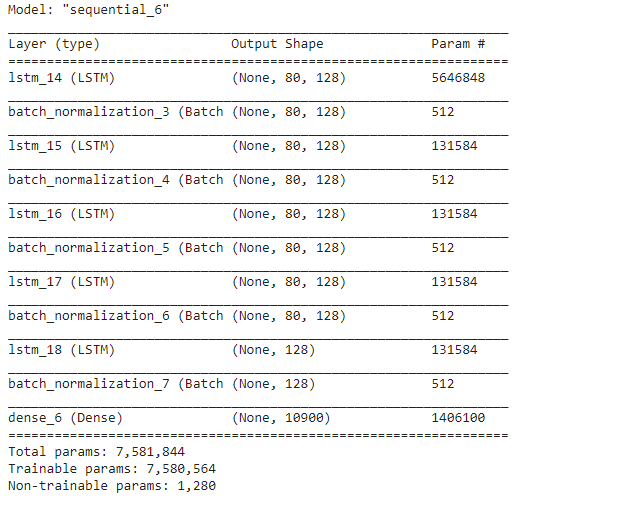
\includegraphics{model2}
The fourth model is the one I got the best results with, using five LSTM layers with Batch Normalization after each layer, as seen above. This model ended up producing the best results, and converging to the lowest loss. A text sample from this model follows:
\\ \\
And now look at a great veterans, it's all a it, first
 like it should better to the great superpower are going to keep fantastic plan taught
 to a Supreme supplies deaths in cash. We destroyed the Brett Supreme
\\
Unfortunately this still isn't very coherent obviously, but it ended up producing text more akin to what Trump would say than the initial models did. One of the major issues with this model and the others was the overfitting due to poor training data size. The loss progress for this model can be seen in the following graph: \\
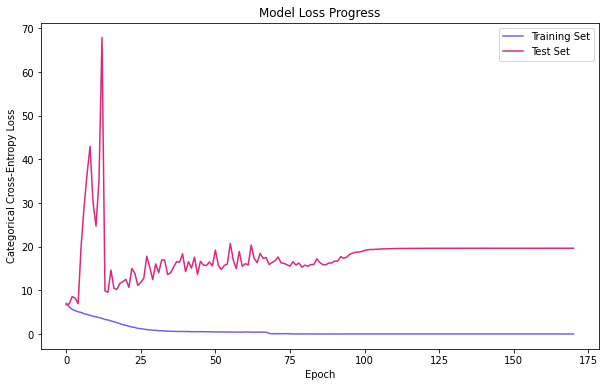
\includegraphics{loss}

This makes it clear that the model is blatantly overfitting, as the loss is going very low while the validation loss is not decreasing. This was due to the lack of sequences, as the likelihood for the unseen test data to contain a sequence that is very similar to sequences in the training data isn't very high. There are many more unseen valid sequences of words spoken by Donald Trump than there are sequences seen by the model, so reducing the validation loss was incredibly difficult with the low amount of RAM available on the colabs runtime.

\section {Discussion}
It's important to discuss ethical considerations when dealing with the topic of AI-generated content mimicking a person. This project was done purely for educational purposes, not to encourage use of data mining techniques to impersonate or slander any person or group of people. Projects like these shouldn't be used to create impersonations or forgeries, as in most places of the world it's probably illegal, and it's unethical regardless.\\

\noindent
While the results for my model weren't as good as I anticipated originally, this project helped me come to understand some of the difficulties of working with a text data set and building sequence based models. With a larger resource pool, it may have been possible to improve performance especially in the case of validation loss. I ended up using techniques for reducing learning rate on plateau and early stopping focused on the actual loss and not the validation loss, as the validation loss wouldn't go down and training would be cut short. One of the interesting things that the better performing models did was that they'd almost always predict a word with a capital letter after a period ending the previous sentence, which was due to punctuation being treated as separate words as mentioned earlier.

\section {Conclusion}
In conclusion, this project details a few attempts at creating an LSTM-based deep learning model for text generation based on the presidential speeches of Donald Trump

\footnotesize
\begin{thebibliography}{99}
\bibitem{Z} Ziang Xie, P. 2017. Neural Text Generation: A Practical Guide. \emph{CoRR.}
\bibitem{SS} Dipti Pawade, Avani Sakhapara, Mansi Jain, Neha Jain, Krushi Gada, P. 2018. Story Scrambler - Automatic Text Generation Using Word Level RNN-LSTM. \emph{I.J. Information Technology and Computer Science.}
\bibitem{C} Sivasurya Santhanam, S. 2020. Context based Text-generation using LSTM networks. \emph {arXiv preprint arXiv:2005.00048.}
\bibitem{VAE} Stanislau Semeniuta, Aliaksei Severyn, Erdhart Barth, P. 2017. A Hybrid Convolutional Variational Autoencoder for Text Generation. \emph{arXiv:1702.02390}
\bibitem{GAN} William Fedus, Ian Goodfellow, Andrew M. Dai, P. 2018. MaskGAN: Better Text Generation via Filling in the \_\_\_ . \emph{arXiv:1801.07736}
\bibitem{CL} Zachary C. Lipton, Sharad Vikram, Julian McAuley, P. 2016. Generative Concatenative Nets Jointly Learn to Write and Classify Reviews \emph{arXiv:1511.03683}
\end{thebibliography}

\end{document}
